
%(BEGIN_QUESTION)

Denne smelteovnen har et kaskadekoblet reguleringssystem der den primære regulatoren måler temperaturen i metallet som er smeltet og sekundær regulatoren regulerer temperaturen i ovnens vegger og tak. 

%This metal-melting furnace has a cascade control system, whereby a ``bath'' controller (sensing the temperature of the molten metal) acts as the primary, and a ``crown'' controller (sensing the temperature of the refractory wall and roof) acts as the secondary:

$$\includegraphics[width=15.5cm]{i01530x01.eps}$$

En dag blir sensorn i TT-1 defekt. Dette gjør at TT-1 sender et signal på 20.6mA. Hvilken effekt vil dette ha på reguleringssystemet?

%One day the crown thermocouple (the sensor for TT-1) goes bad, causing TT-1 to ``fail high'' with a 20.6 mA signal.  Determine the effect(s) this will have on the control system as a whole, and on the furnace temperature in particular.

\vskip 10pt


\begin{tikzpicture}
	\draw[step=0.5cm,gray!20,very thin]  grid (16,10) ;
\end{tikzpicture}

\vskip 20pt \vbox{\hrule \hbox{\strut \vrule{} {\bf Suggestions for Socratic discussion} \vrule} \hrule}

\begin{itemize}
\item{} Determine the necessary control actions (direct vs. reverse) for each controller in this system, assuming a signal-to-open valve.
\item{} Why do you think a cascade control strategy is used to control the burner?
\item{} For those who have studied thermocouples, what {\it type} (letter code) of thermocouple would you recommend for this application, assuming a crown temperature upwards of 1800 $^{o}$F?
\end{itemize}

\underbar{file i01530}
%(END_QUESTION)





%(BEGIN_ANSWER)

Not having the thermocouple fully inserted into the thermowell leads to additional {\it lag time}, as the air gap between the thermocouple tip and the thermowell bottom generates a time lag between the thermowell temperature and the thermocouple tip temperature. 

%(END_ANSWER)





%(BEGIN_NOTES)

A ``high burnout'' TT-1 would cause the furnace to cool down, as the temperature control system would ``think'' the furnace was too hot and take the necessary action of stopping heat input.

\vskip 10pt

Specifically, lag time in a feedback control system leads to greater phase shift, which may result in oscillation (cycling) given enough controller gain.  This is quite common in temperature control applications such as this, where the process itself may have only one dominant lag, allowing aggressive proportional action from the controller to achieve tight, fast control.  The addition of more lag times in a loop like that will often lead to oscillation, as the high gain of the controller now has enough phase shift to complement it and meet (or exceed) the Barkhausen criterion.

\vfil \eject

\noindent
{\bf Prep Quiz:}

An thermocouple improperly inserted into its thermowell can cause control problems by introducing what characteristic to the temperature control loop?

\begin{itemize}
\item{} Integral action
\vskip 10pt
\item{} Stiction
\vskip 10pt
\item{} Hysteresis
\vskip 10pt
\item{} Positive error
\vskip 10pt
\item{} Extra lag time
\vskip 10pt
\item{} Reverse action
\end{itemize}


%INDEX% Control, strategies: cascade with limits
%INDEX% Process: combustion furnace

%(END_NOTES)


